\begin{figure}\centering
	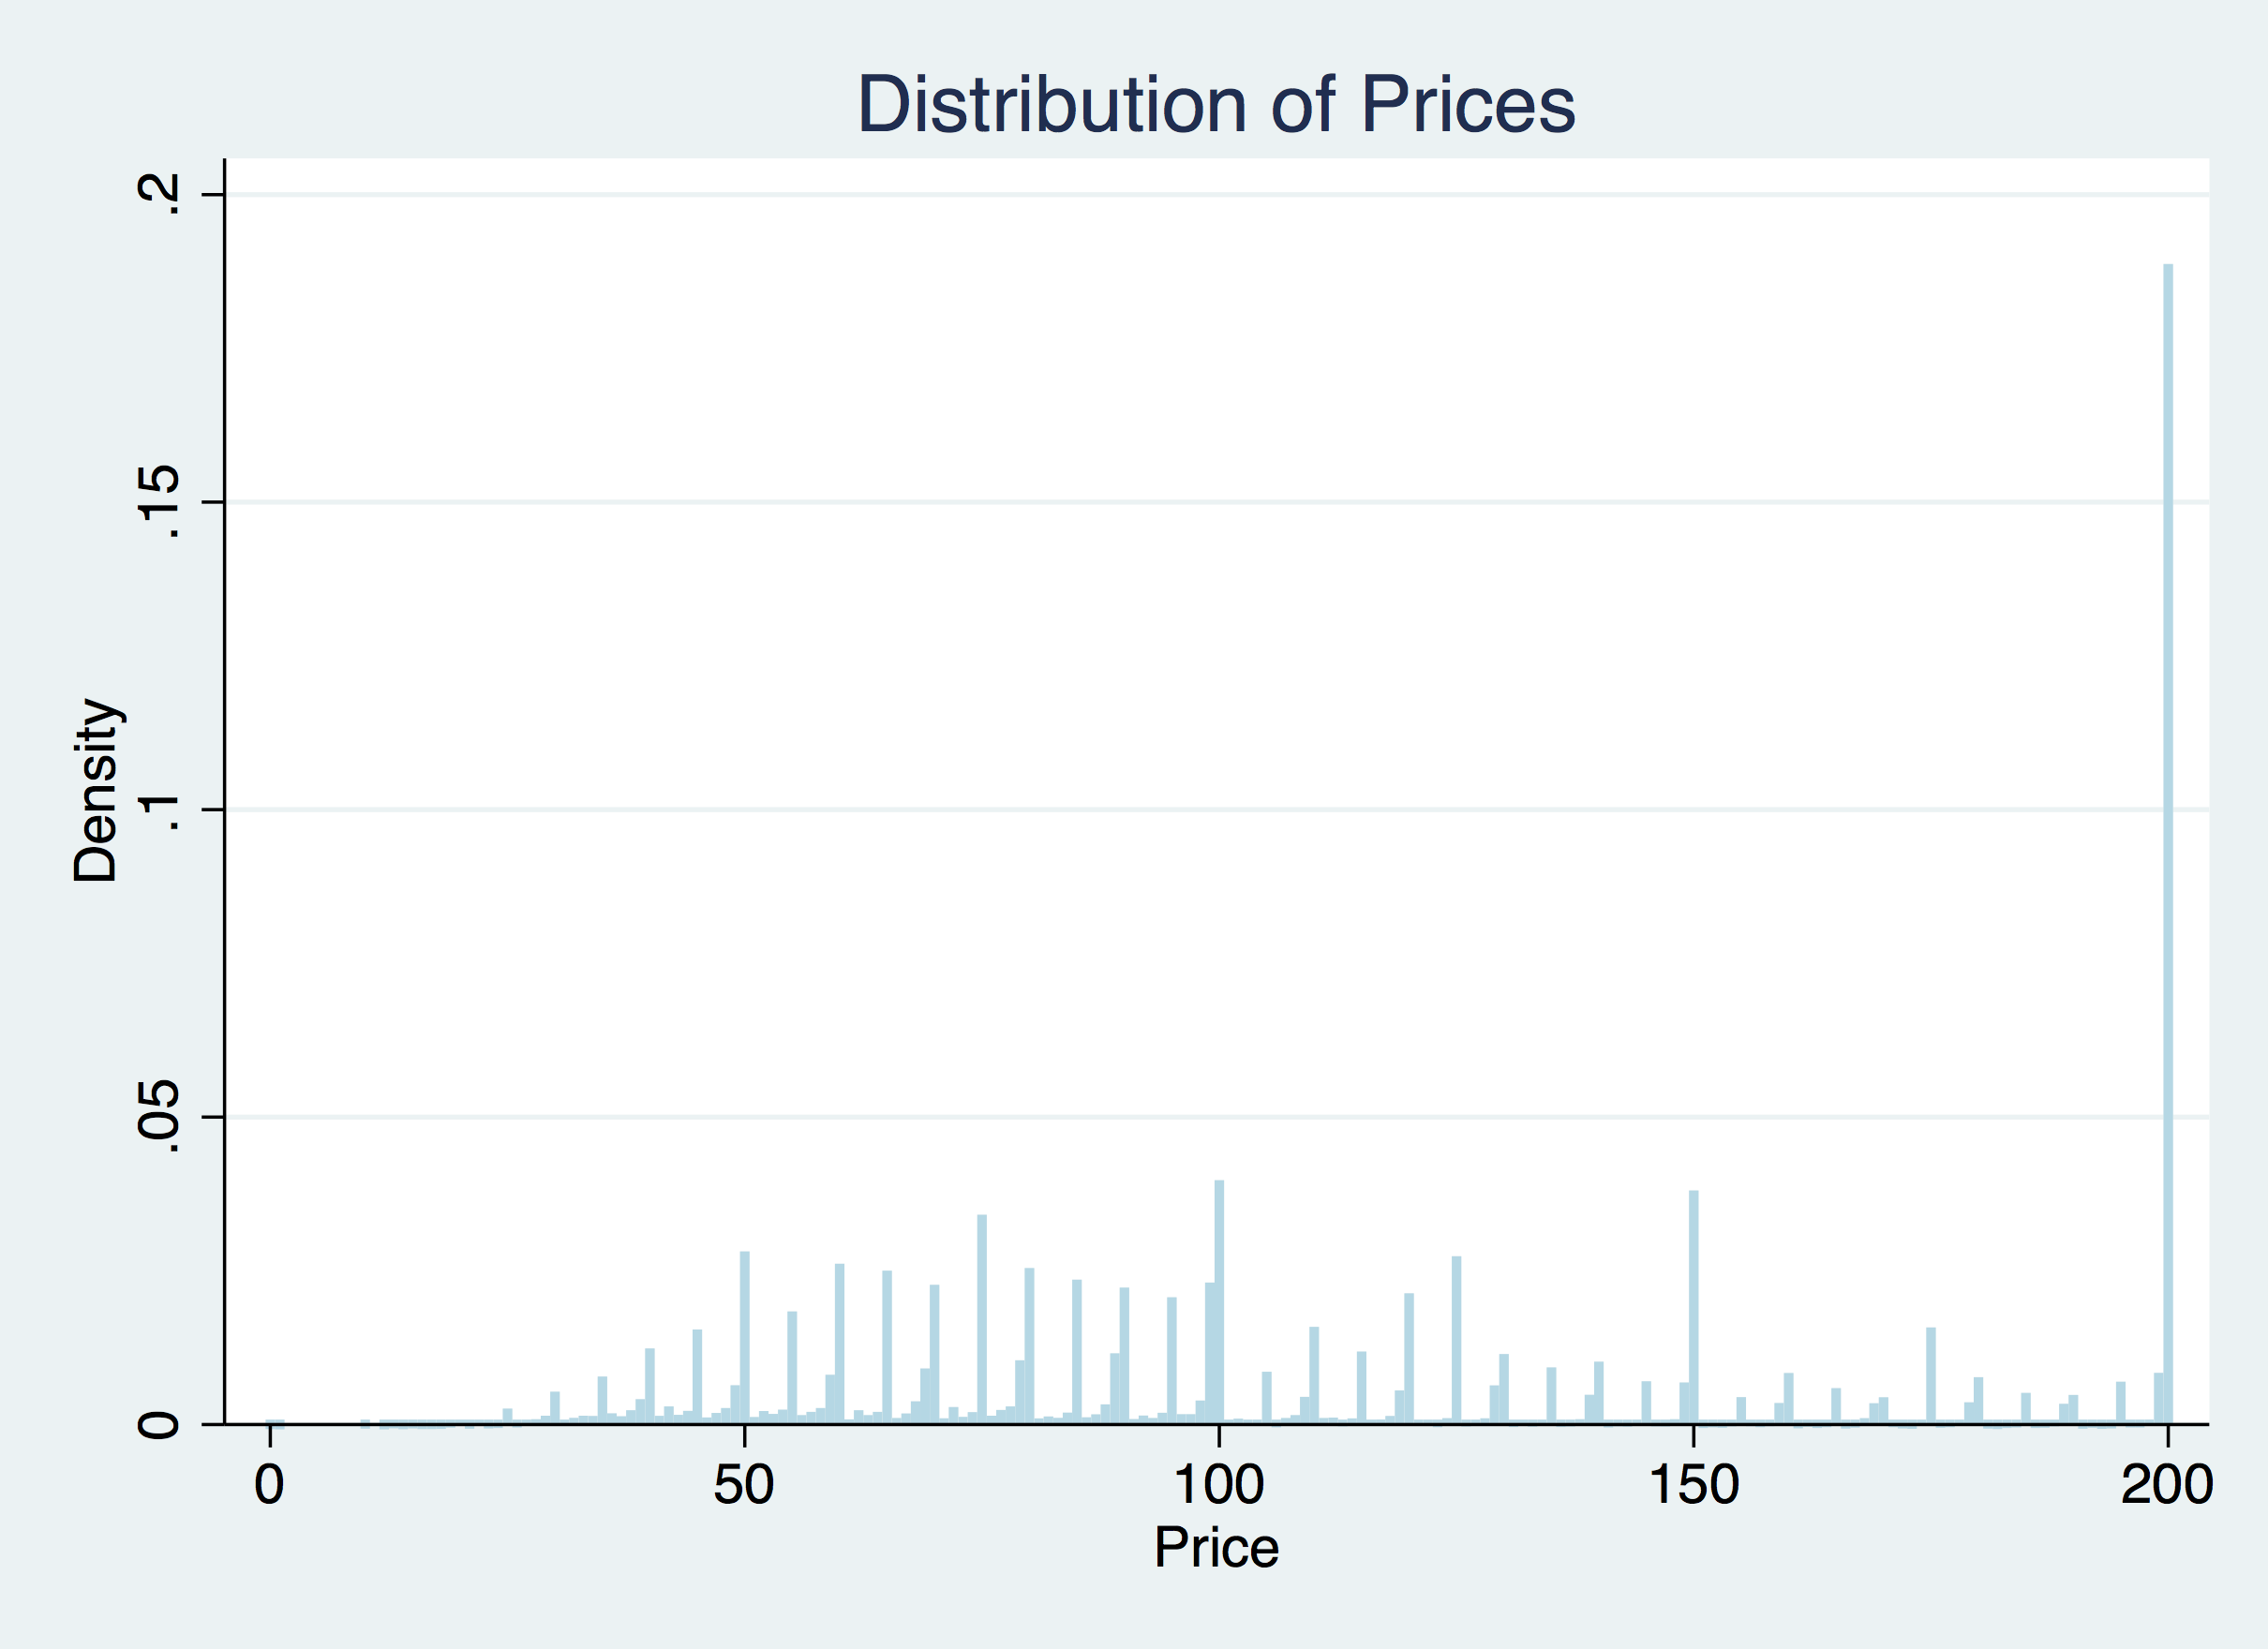
\includegraphics[width=.8\textwidth]{figures/price_dist-DISC-100}
	\caption{Distribution of prices}
	\caption*{Notes: All the offerings priced at \$200 or more are grouped together at price = 200}
\end{figure}
\begin{figure}\centering
	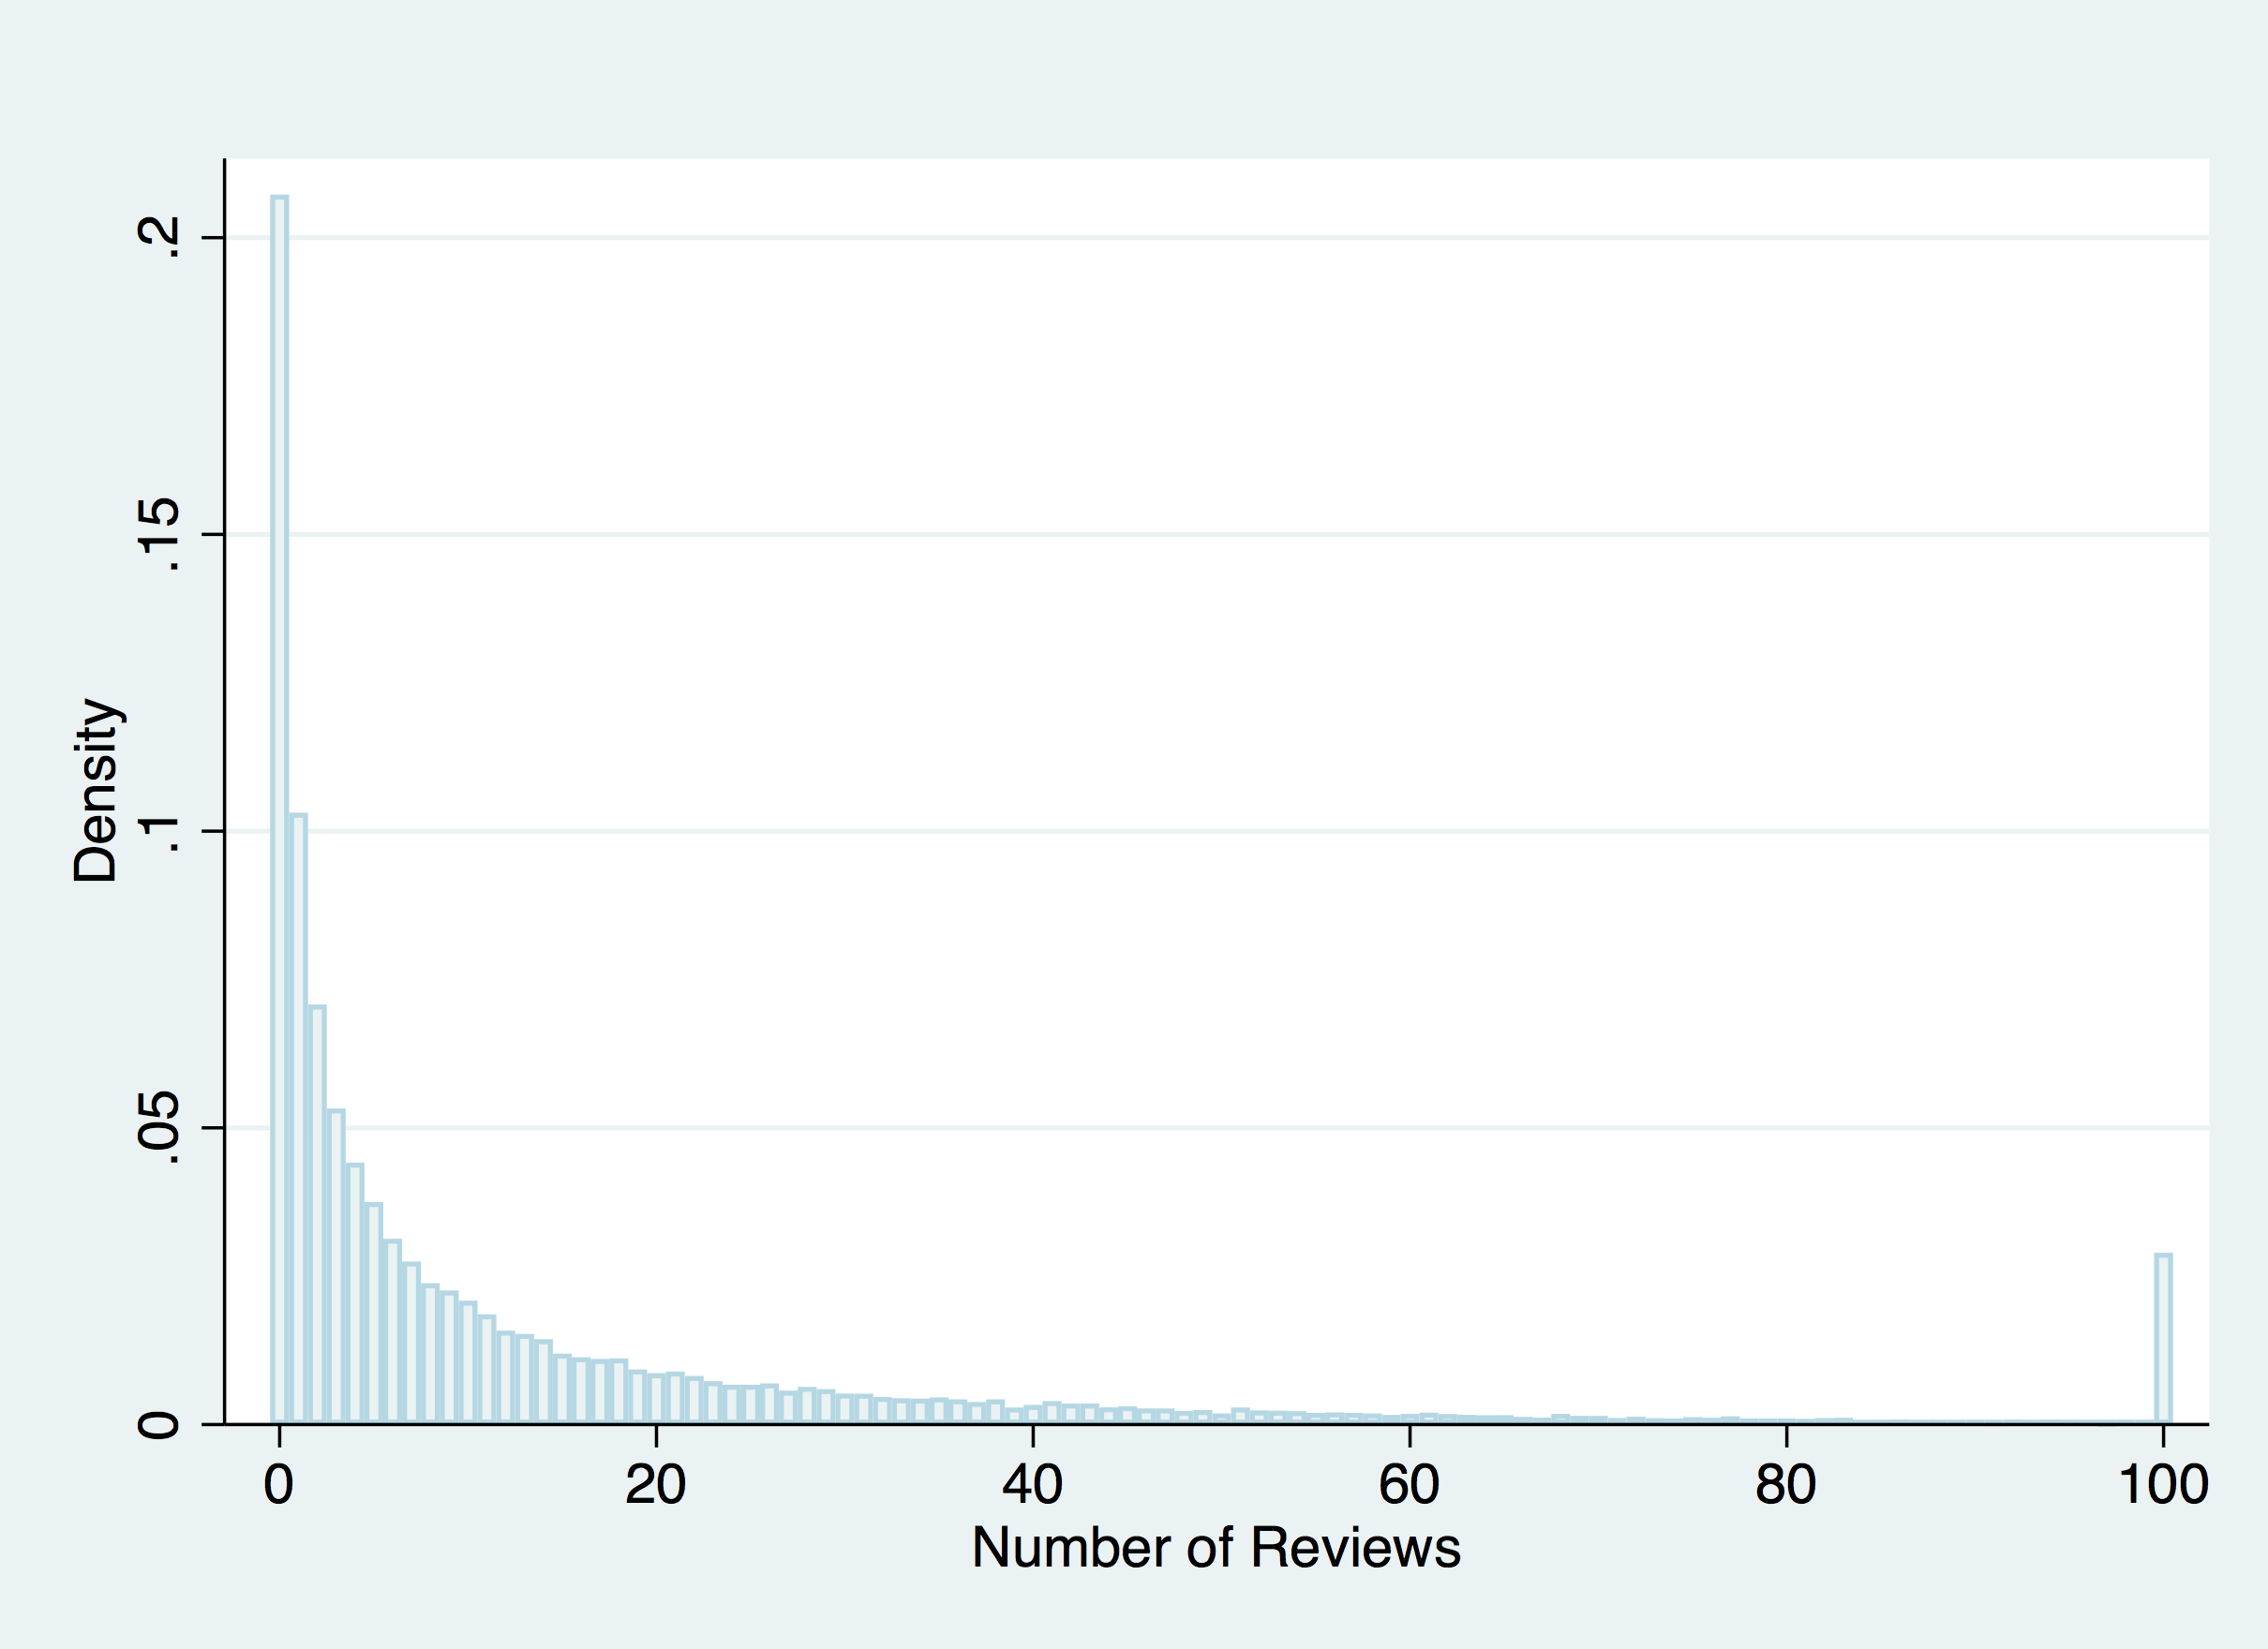
\includegraphics[width=.8\textwidth]{figures/num_reviews_dist-DISC-100}
	\caption{Distribution of number of reviews}
	\caption*{Notes: All the offerings with 100 reviews or more are grouped together at number of reviews = 100}
\end{figure}
\begin{figure}\centering
	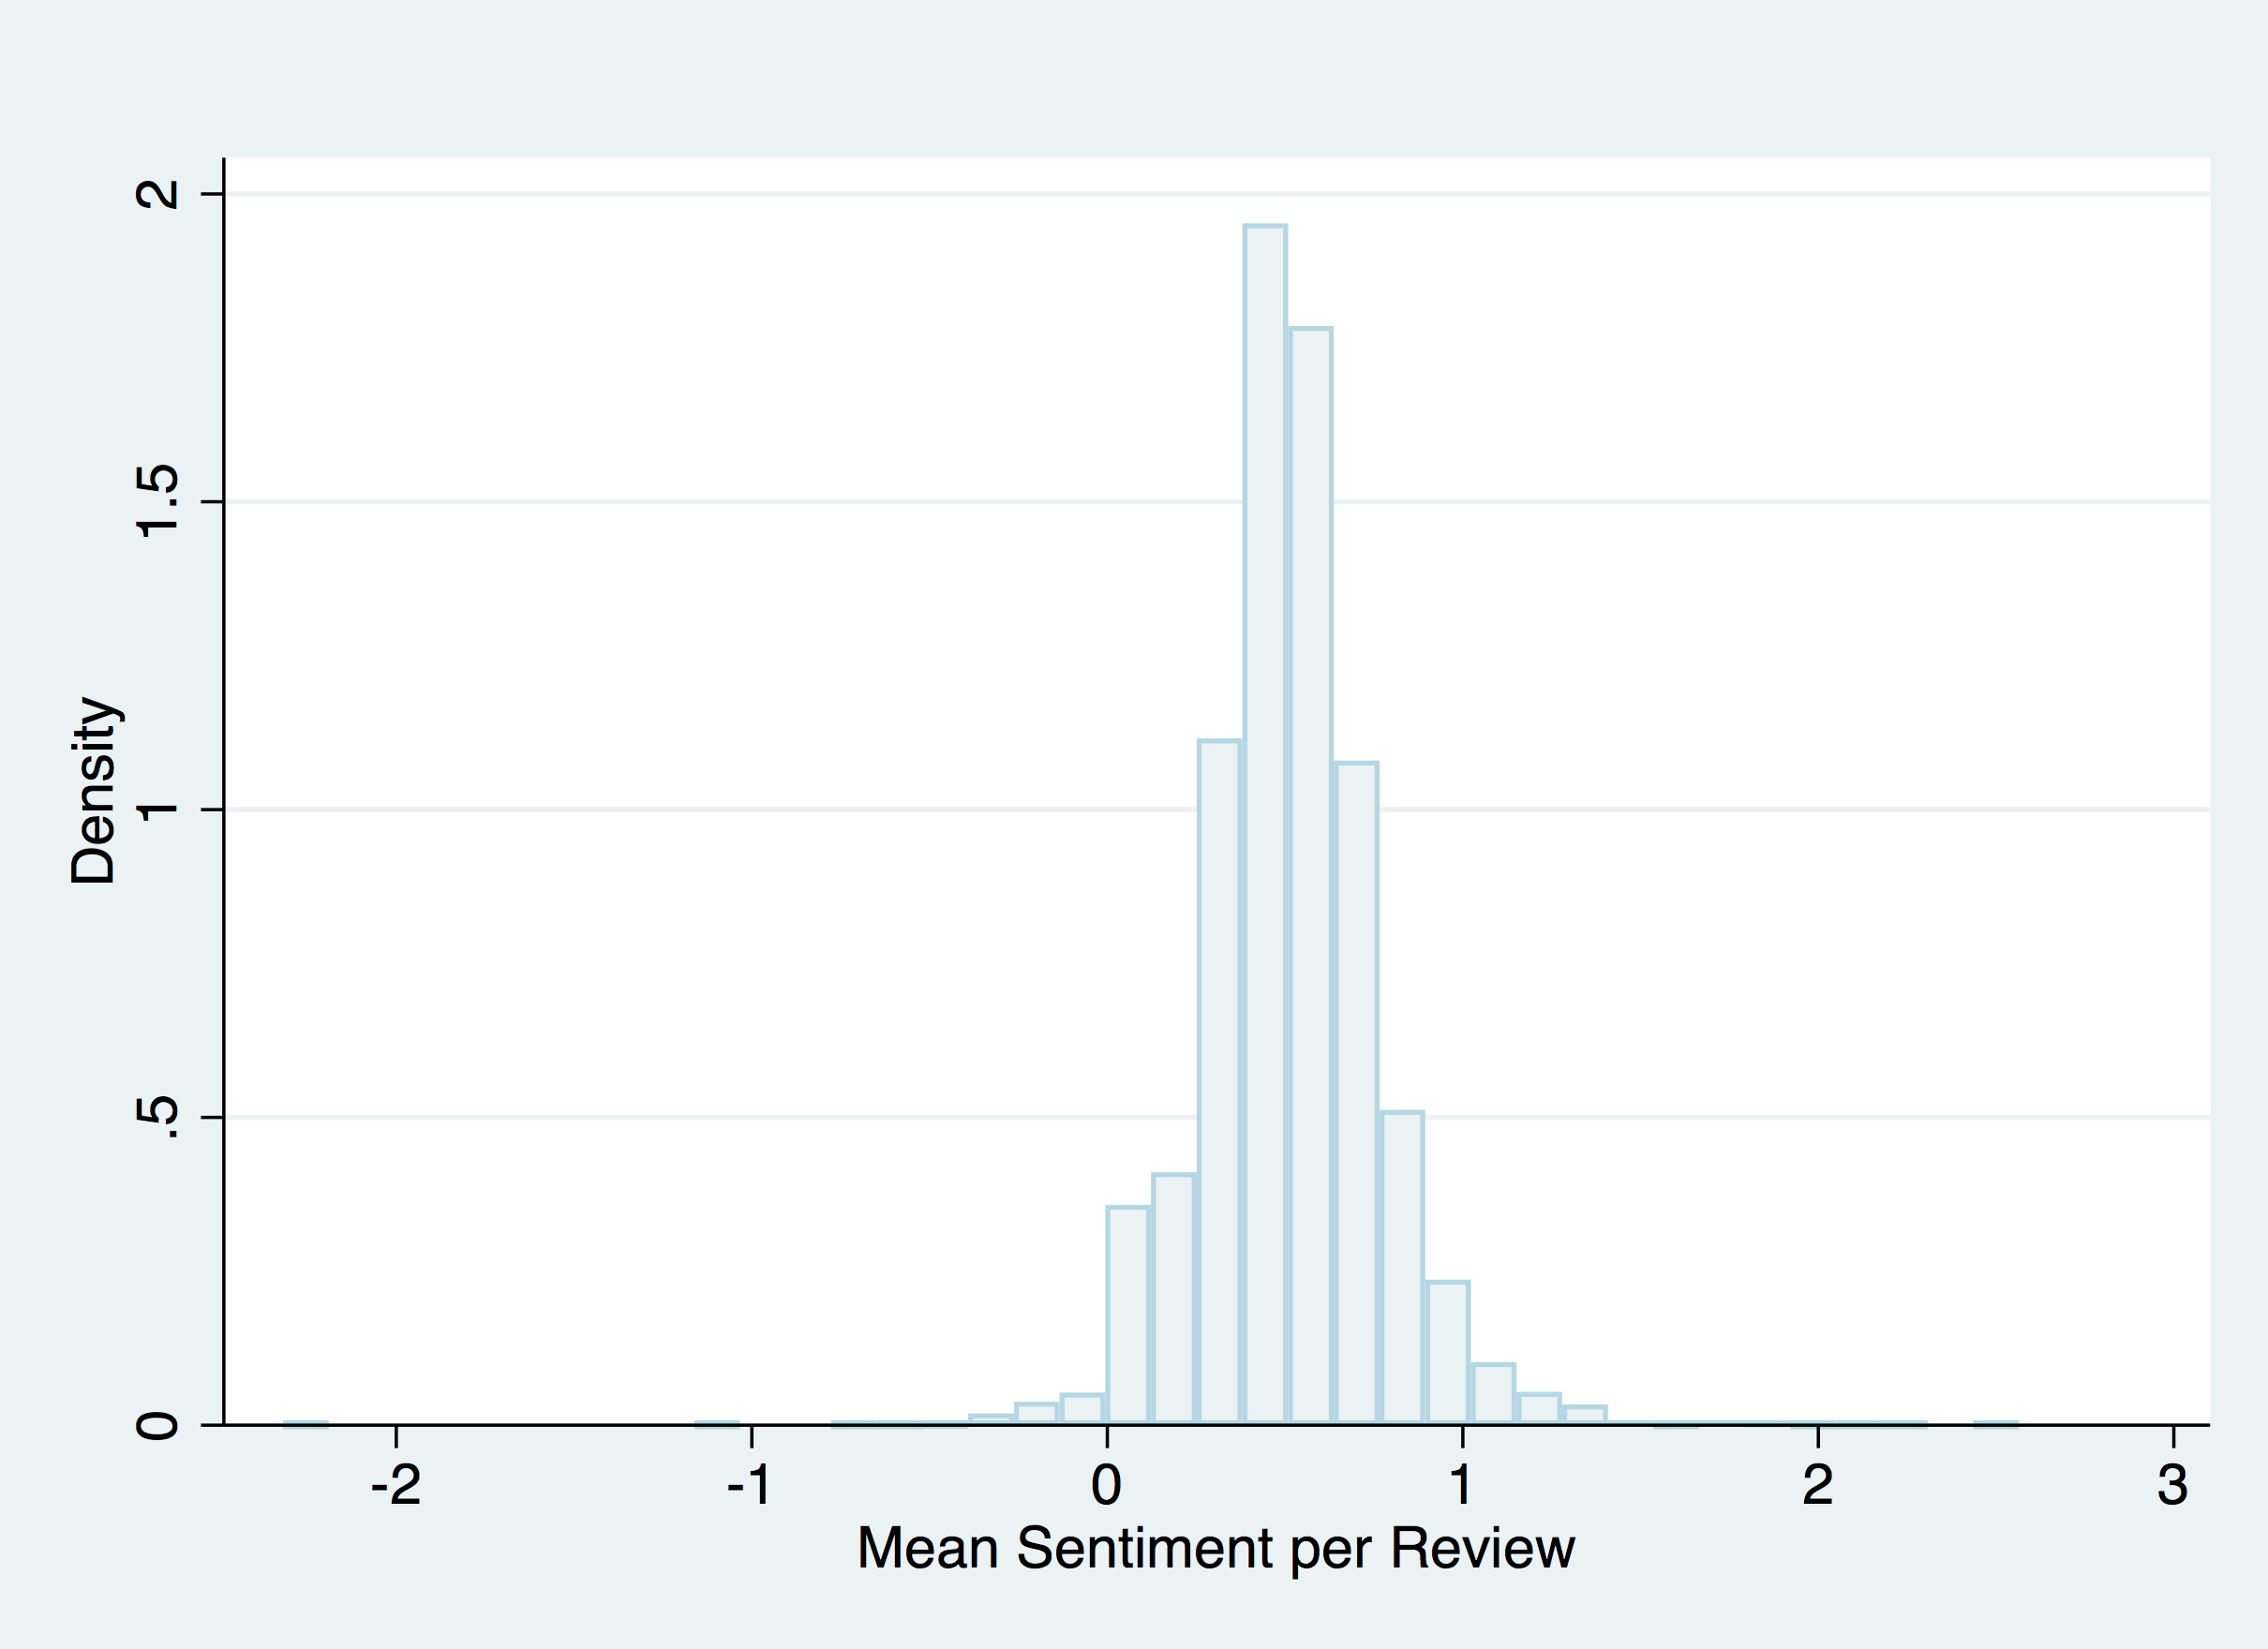
\includegraphics[width=.8\textwidth]{figures/review_sentiment_dist}
	\caption{Distribution of review sentiment}
\end{figure}
\begin{figure}\centering
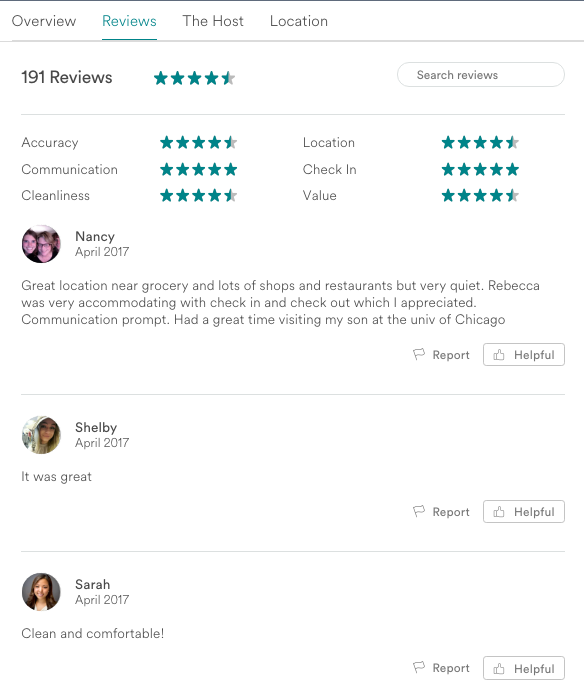
\includegraphics[width=.8\textwidth]{figures/sample3-reviews}
\caption{Sample review information}
\end{figure}
\begin{figure}\centering
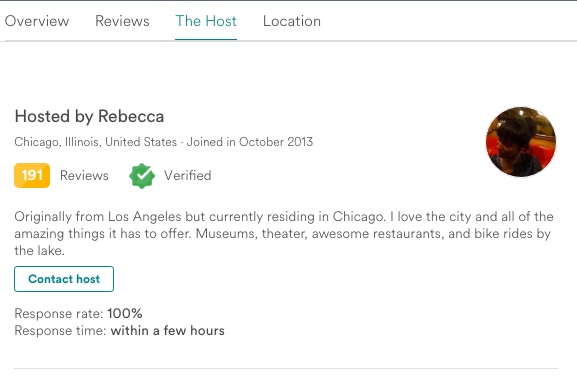
\includegraphics[width=.9\textwidth]{figures/sample4-host}
\caption[Sample host information]{Sample host information available. Note that this Figure reflects the changes made to the website after Airbnb updated its discrimination policy. The guests in my data would have seen a larger host profile picture than shown here.}
\end{figure}
\begin{figure}\centering
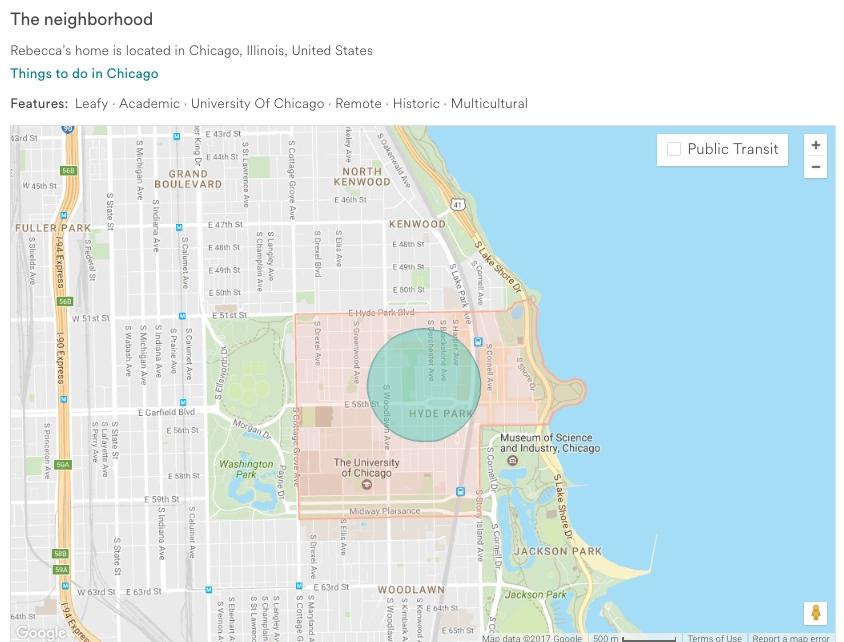
\includegraphics[width=.8\textwidth]{figures/sample5-location}
\caption{Sample location information}
\end{figure}
\begin{figure}\centering
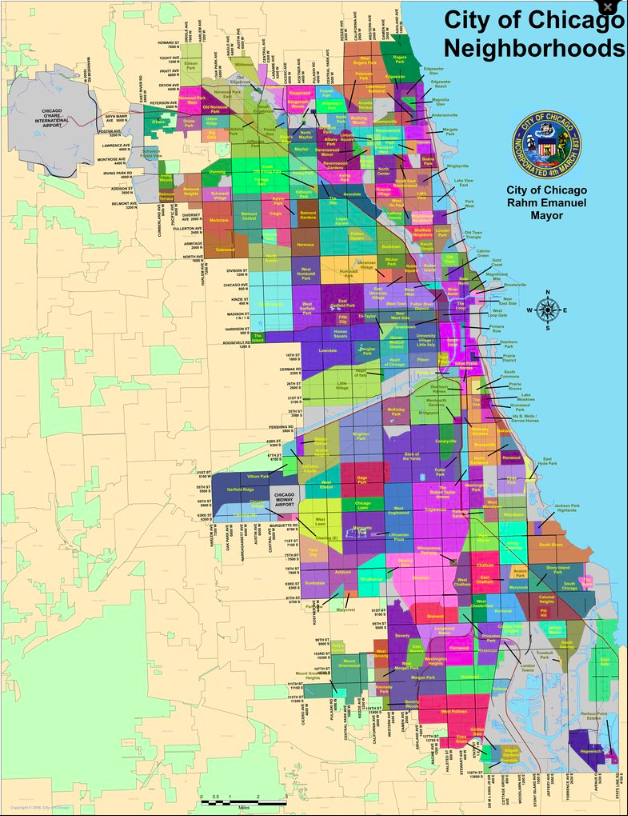
\includegraphics[width=.8\textwidth]{figures/chicago_city_neighborhoods}
\caption[City of Chicago neighborhoods]{City of Chicago neighborhoods, showing level of granularity of neighborhood controls}
\end{figure}


